\chapter{Security configuration of Norwegian operators}
\label{chap:security_configuration_of_norwegian_operators}

\iffalse

    Dev these
    attacks, test if it works! Insist on the product, no other
    publication gives this level of detail in the security of norwegian
    network. A bit in decoding gsm but almost nothing. try to explain
    the method and give it a nice name. about the method, talk about
    gsmmap and maybe analyze their method. how i tried to solve the pb
    and gather the data.

\fi
  The goal of this chapter is, using \proj{OsmocomBB}, to take a look at
  the security configuration of Norwegian mobile network operators. The
  attacks introduced in~\Cref{chap:eavesdropping_attacks}
  and~\Cref{chap:dos_attacks} will be investigated, as long as they do
  not disturb the normal operation of the networks.

  The first section of this chapter is dedicated to practical
  considerations about the gathered data. The second section
  investigates the eavesdropping attack described
  in~\Cref{chap:eavesdropping_attacks} by considering each assumption
  it makes. The last section does the same for the \gls{dos} attacks
  introduced in~\Cref{chap:dos_attacks}.

  \section{Data gathering}

    The data gathered for this thesis is the result of relatively simple
    tests on a limited number of cells around the \gls{ntnu} Gløshaugen
    campus. The scope of the results and conclusions is thus limited.
    These experiments are intended as an exploration of the feasibility
    of the attacks described in this thesis, and are by no means an
    extensive investigation. For an analysis on a larger scale, the
    \proj{GSM Map} project is interesting.

    The \proj{GSM Map} project  aims to gather security configuration
    data samples submitted by volunteers from all over the world and to
    use it to assess mobile networks security. It creates automatically
    generated reports presenting this information and publish them
    online~\cite{security_research_labs_gsm_????}. However, since the
    reports are not reviewed before publication, the analysis they offer
    does not claim accuracy. Moreover, the number of samples and the
    date of submission are not available. These reports are thus useful,
    but should not be used to draw conclusions on their own. Therefore,
    the data gathered here will also be compared to the \proj{GSM Map}
    report dedicated to
    Norway~\cite{security_research_labs_mobile_2015}. This is a way to
    verify their claim, but also to back up the results found here.

    The measures were done using various \gls{sim} cards: one from
    \comp{Telenor}, one from \comp{Netcom}, one from \comp{Base}, and
    two from \comp{Proximus}. \comp{Telenor} and \comp{Netcom} are two
    Norwegians operators, while \comp{Proximus} and \comp{Base} are two
    Belgian operators. Unfortunately, the \comp{Telenor} \gls{sim}
    crashes the phones when used with \proj{OsmocomBB}, and the
    \comp{Netcom} \gls{sim} is simply not recognized by any of the
    available compatible phones, using \proj{OsmocomBB} or not. This
    means that a \comp{Proximus} \gls{sim} roaming on \comp{Netcom}, as
    well as a \comp{Base} \gls{sim} roaming on \comp{Telenor} were used
    for the experiments involving \proj{OsmocomBB}. All the \gls{sim}
    cards worked fine on a \comp{Samsung Galaxy Mini 2} phone running
    \comp{Android} $2.3.6$ which was used when possible.\fxnote{what are
      the implication of roaming?}

  \section{Eavesdropping attack}

    The success of the eavesdropping attack introduced
    in~\Cref{chap:eavesdropping_attacks} relies on several assumptions.
    Firstly, that it is possible to perform an \gls{hlr} query.
    Secondly, that the \gls{tmsi} is not reallocated when an \gls{sms}
    message is received. Thirdly, that it is possible to send silent
    \gls{sms} messages. Fourthly, that the encryption used is breakable.
    And finally, that it is possible to find known plaintext. Each of
    these assumptions will be investigated.
    \Cref{chap:eavesdropping_attacks} also introduces other abuses of
    the \gls{ss7}, but this could not be investigated since it requires
    an access to this network. 

    \subsection{HLR query}

      The first step is to make sure that HLR queries return valid
      results on Norwegian networks. Since \proj{OsmocomBB} is not
      needed for this first step, all the available \gls{sim} cards can
      be used. As explained in~\Sref{sec:sriforsm}, based on a phone
      number, an \gls{hlr} query returns the related \gls{imsi}, and the
      number of the Serving \gls{msc}. An online service allowing to
      query the \gls{hlr} using various routing options was
      used~\cite{hlr_lookup}. Depending on the route, the query returned
      different parameters. For example, one route returns the
      \gls{imsi} but not the \gls{msc} number, while it is the opposite
      for another. The experiments were done three times, with a few
      days interval between each session. Each request was fired at
      least three times per session, using every available routing
      option. The output of the Web Client available on this service is
      displayed on~\fref{fig:hlr_lookup}.

      \begin{figure}[h]
        \centering
        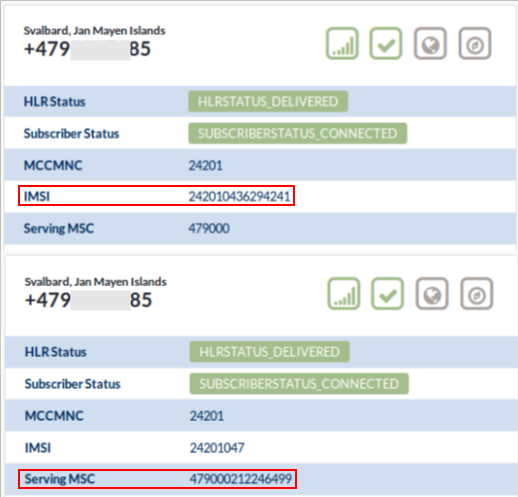
\includegraphics[width=.7\textwidth]{hlr_lookups_both}
        \caption{Result of an HLR query, displaying the IMSI on the
        top, and the MSC number on the bottom~\cite{hlr_lookup}}
        \label{fig:hlr_lookup}
      \end{figure}
      
      Using this service, both Norwegian networks return a fake
      \gls{imsi}. Even though it is trivial to compare the returned
      \gls{imsi} with the actual one, it is more difficult to assess the
      validity of the Serving \gls{msc} number. For \comp{Telenor}, this
      number seems random, as it is different in every request result.
      For \comp{Netcom}, it is constant in time and has a Norwegian
      prefix, which makes the result more plausible. 
      
      For the record, the Belgian operator \comp{Proximus} gives out the
      real \gls{imsi}. It also gives a Serving \gls{msc} number which
      seems correct, since it is stable and has a Norwegian prefix. The
      Belgian operator \comp{Base} gives a fake \gls{imsi}, but the
      results looks similar to \comp{Proximus} for the Serving \gls{msc}
      number. The results of the queries are presented
      in~\tref{tab:hlr_queries}.

      According to the \proj{GSM Map} report, the \gls{imsi} and the
      Serving \gls{msc} number are masked on both Norwegian networks.
      This is consistent with the results presented here. According to the
      report dedicated to Belgium, the \gls{imsi} is masked by every
      Belgian operator, and the Serving \gls{msc} number is masked by
      \comp{Base}, but not by \comp{Proximus}, which is not consistent
      with the results presented
      here~\cite{security_research_labs_mobile_2015-1}. 
      
      \begin{table}[h]
        \centering
        \begin{tabular}{@{}lll@{}}
          \toprule
          Operator             & Correct IMSI & Serving MSC\\
          \midrule
          Telenor              & No   & random     \\
          Netcom               & No   & 4792001019 \\
          Base (On Telenor)    & No   & 4741713899 \\            
          Proximus (On Netcom) & Yes  & 4792003990 \\
          \bottomrule
        \end{tabular}
        \caption{Results of the HLR queries.}
        \label{tab:hlr_queries}
      \end{table}
      
      These results are good for both \comp{Telenor} and \comp{Netcom}
      because the \gls{imsi} can be used in various attacks, for example
      in the \gls{imsi} detach \gls{dos} attack. It is not clear if
      \comp{Netcom} leaks the real Serving \gls{msc} number, but it is
      not an essential part of the eavesdropping attack anyway. Indeed,
      the location of the target can be found by other means.

      \iffalse

      Telenor, no problem. +4791xxxx85
      IMSI 242013977953009/24201311xxxxx91 clearly random
      serving msc 479000213040191 seems ok but louche
      serving hlr 4790000947 seems ok
      The imsi changes with each request, but the serving stay the same

      Proximus roaming netcom, no problem +32477646158
      206012220938542 / 20601xxxx938542
      serving msc 4792003990
      serving hlr 32477646158
      stays the same with each request

      Proximus netcom +32479xxxx15
      206012219452575/206012219452575  
      serving msc 4792002001 seems stable
      serving hlr 32479755215

      Chess (MVNO netcom), +47471xxxx5 (virtual operator can have different stuff…)
      query: 24202747143405 (fake but not random) true: 24202560xxxx342
      4792001019 constant, seems ok
      4792001032 (increments…)

      Base roaming telenor
      2062094588440 / 2062010xxxx9724 (with xt5 get 2060100)
      4741713899 xt5
      32494588440 (with xt5 get 324860)
      \fi

    \subsection{Silent SMS messages}
    \label{sec:silent_sms}

      Uncovering the targeted phone \gls{tmsi} and location can be done
      through a correlation between Paging Request messages in a
      location area and \gls{sms} messages sent to the targeted phone,
      as explained in~\Sref{sec:recovering_tmsi}. To avoid raising
      suspicion from the targeted user, it is possible to exploit so
      called silent \gls{sms} messages by setting the TP-PID and TP-DCS
      fields in the header~\cite[p.~53]{3gpp_ts_2001}.
      
      Some networks filter these fields as a security feature, and set
      the bytes back to \code{0x00} when the TP-PID field was set to
      \code{0x40} and the TP-DCS field was set to \code{0xC0}. This can
      be tested using \proj{OsmocomBB} by slightly modifying its code
      using the \prog{silent} command developed for this thesis and
      introduced in \Sref{sec:recovering_tmsi}. Upon reception of these
      silent \gls{sms} messages, the receiving phone is paged and the
      transaction on the dedicated channel occurs normally, which makes
      it possible to read the two fields on both side of the
      communication using \proj{Wireshark}. This can only be done with
      the \comp{Proximus} and \comp{Base} \gls{sim} cards roaming on
      \comp{Netcom} and \comp{Telenor} respectively, since
      \proj{OsmocomBB} is needed. The results are displayed in
      \tref{tab:silent_sms_traffic}. \fref{fig:silent_sms_tx} and
      \fref{fig:silent_sms_rx} show the values of these fields in
      Wireshark when sent from the \comp{Netcom} network and received on
      the \comp{Telenor} network respectively.

      \begin{table}[h]
        \centering
        \begin{tabular}{@{}lll@{}}
          \toprule
          \multirow{2}{*}{Recipient} & \multicolumn{2}{c}{Sender}   \\
          \cmidrule(l){2-3}
                            & Telenor (Base)    & Netcom (Proximus) \\
          \midrule
          Telenor (Base)    &                   & \code{0x00} and \code{0xC0} \\
          Netcom (Proximus) & \code{0x40} and \code{0xC0} &                   \\
          \bottomrule
        \end{tabular}
        \caption{Received values of the TP-PID and TP-DCS fields
          when sent set to \code{0x40} and \code{0xC0} respectively}
        \label{tab:silent_sms_traffic}
      \end{table}

      \begin{figure}[t]
        \centering
        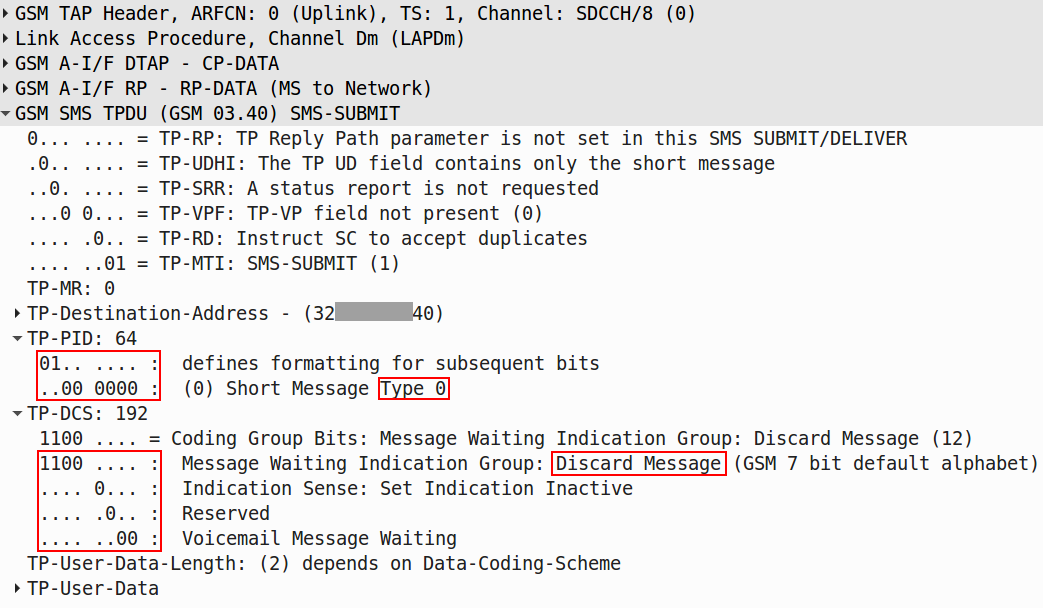
\includegraphics[width=\textwidth]{silent_sms_tx}
        \caption{Sent TP-PID and TP-DCS fields from \comp{Netcom}}
        \label{fig:silent_sms_tx}
      \end{figure}

      \begin{figure}[t]
        \centering
        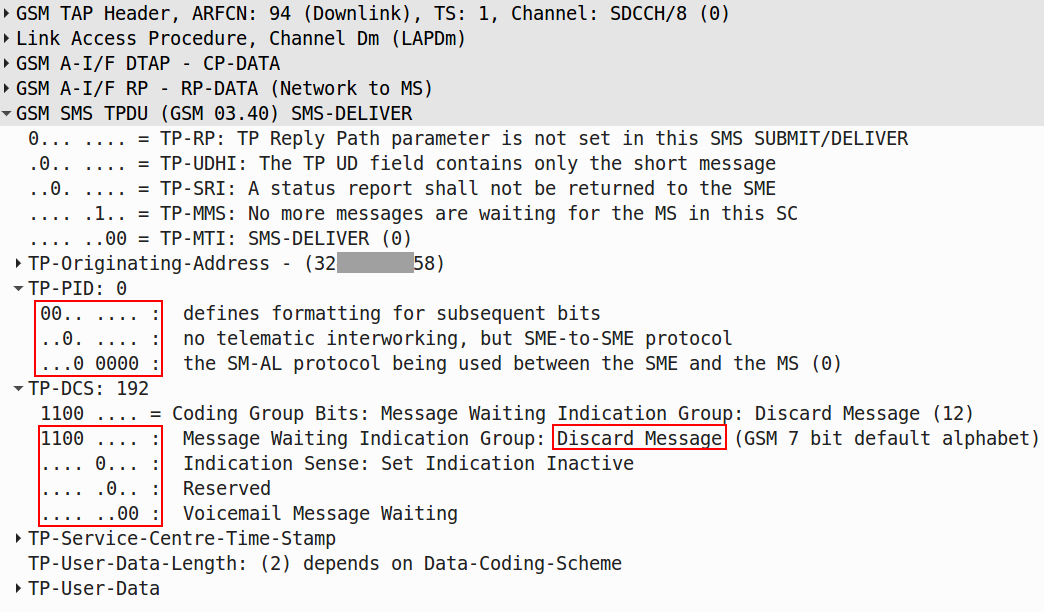
\includegraphics[width=\textwidth]{silent_sms_rx}
        \caption{The received TP-PID and TP-DCS fields on
        \comp{Telenor} are filtered}
        \label{fig:silent_sms_rx}
      \end{figure}

      \iffalse
      The TP-PID field is filtered either by \comp{Telenor} on
      reception, or by \comp{Netcom} on sending. Need to find a second
      \comp{Telenor} \gls{sim} to make sure of that. Also need to try
      sending from on \comp{Netcom} \gls{sim} to the other. I need to
      test that a bit more and to check all the values again. I need to
      have two true Telenor sims and two true Netcom sims which work
      with OsmocomBB.\fxnote{fixme!}
      \fi

      To complete these tests, some \gls{sms} messages were sent from
      the two phones running \proj{OsmocomBB} with the \comp{Proximus}
      and \comp{Base} \gls{sim} cards to the modern phone running
      \proj{Android} with all the available \gls{sim} cards in turns. It
      was not possible to observe the traffic in this case, but the
      point is to determine if the receiving phone alerts the user. The
      results are shown on~\tref{tab:silent_sms_notification}.

      \begin{table}[h]
        \centering
        \begin{tabular}{@{}lll@{}}
          \toprule
          \multirow{2}{*}{Recipient} & \multicolumn{2}{c}{Sender}   \\
          \cmidrule(l){2-3}
                            & Telenor (Base)    & Netcom (Proximus) \\
          \midrule
          Telenor           & Yes               & No                \\
          Netcom            & Yes               & No                \\
          Telenor (Base)    &                   & No                \\
          Netcom (Proximus) & Yes               & No                \\
          \bottomrule
        \end{tabular}
        \caption{Notification of the user when the TP-PID and TP-DCS
        fields were sent set to \code{0x40} and \code{0xC0}
      respectively}
        \label{tab:silent_sms_notification}
      \end{table}
      
      From these results, we can conclude that \comp{Telenor} filters
      the TP-PID field on reception while \comp{Netcom} does not. This
      makes silent \gls{sms} messages ineffective on the \comp{Telenor}
      network while it is effective on the \comp{Netcom} network. Other
      methods could be used to page an \gls{ms} without alerting the
      user, and they are described in~\Sref{sec:recovering_tmsi} but
      were not tested here. Also, the TP-DCS field seems to not have any
      effect on the user notification.

      \iffalse
      Message sent from Proximus netcom.
      changing tp-pid to 0x40 does not work with proximus on netcom
      changing tp-pid to 0x40 does work with telenor
      changing tp-pid to 0x40 does work with chess
      I receive the ack for successful message, but it would be better
      if I could sniff the traffic to see if it is paged and so on.

      Message sent from Proximus netcom.
      changing tp-pid to 0x40 and the tp-dcs to 0xC0 does work with proximus on netcom
      changing tp-pid to 0x40 and the tp-dcs to 0xC0 does work with telenor
      changing tp-pid to 0x40 and the tp-dcs to 0xC0 does work with chess
      I receive the ack for successful message, but it would be better
      if I could sniff the traffic to see if it is paged and so on.

      Message sent from Proximus netcom.
      changing tp-dcs to 0xC0 does work with chess
      I receive the ack for successful message, but it would be better
      if I could sniff the traffic to see if it is paged and so on.

      I NEED A PURE TELENOR AND NETCOM SIM THAT WORK WITH OSMOCOM…
      \fi

    \iffalse
      http://comments.gmane.org/gmane.comp.mobile.osmocom.baseband.devel/2408
      Hei,
      consider also, that some operators detects silent sms and
      restores automatically TP-PID and TP-DCS.

      Moreover changing TP-PID/TP-DCS I suggest you to use also
      Message Waiting Indication-Discard option [1].

      Some examples: 

      #pdu='0011000C91'+str(num)+'0000AA0141'        # SMS Classic
      #pdu='0011000C91'+str(num)+'4000AA0141'        # 0x40 (TP-PID) 
      #pdu='0011000C91'+str(num)+'40C0AA0141'   # 0x40(TP-PID) and
      0xC0(Message Waiting Indication-Discard)

      Cheers,
      Luca
      \fi


    \subsection{TMSI reallocation}
    \label{sec:tmsi_realloc}

      The \gls{tmsi} reallocation frequency also determines the
      feasibility of the correlation between the Paging Request messages
      and the \gls{sms} messages. If the \gls{tmsi} is reallocated every
      time the targeted \gls{ms} is paged, it is impossible to correlate
      anything. Thus, a good security feature for the networks is to
      reallocate the \gls{tmsi} as often as possible. This can be tested
      by recording the various network events using \proj{OsmocomBB} and
      \proj{Wireshark}. The recorded events were the \glspl{moc}, the
      \glspl{mtc}, the \gls{mo-sms} messages, and the \gls{mt-sms}
      messages, and every measure was taken at least three times. An
      example of an \gls{mt-sms} on \comp{Telenor} is given
      on~\fref{fig:tmsi_real}.

      \begin{table}[h]
        \centering
        \begin{tabular}{@{}lllll@{}}
          \toprule
          Operator          & MTC & MOC & MT-SMS & MO-SMS \\
          \midrule
          Telenor (Base)    & Yes & Yes & Yes    & Yes    \\
          Netcom (Proximus) & Yes & Yes & Yes    & Yes    \\
          \bottomrule
        \end{tabular}
        \caption{TMSI reallocation procedure during various events.}
        \label{tab:events_tmsi_reallocation}
      \end{table}

      \begin{figure}[h]
        \centering
        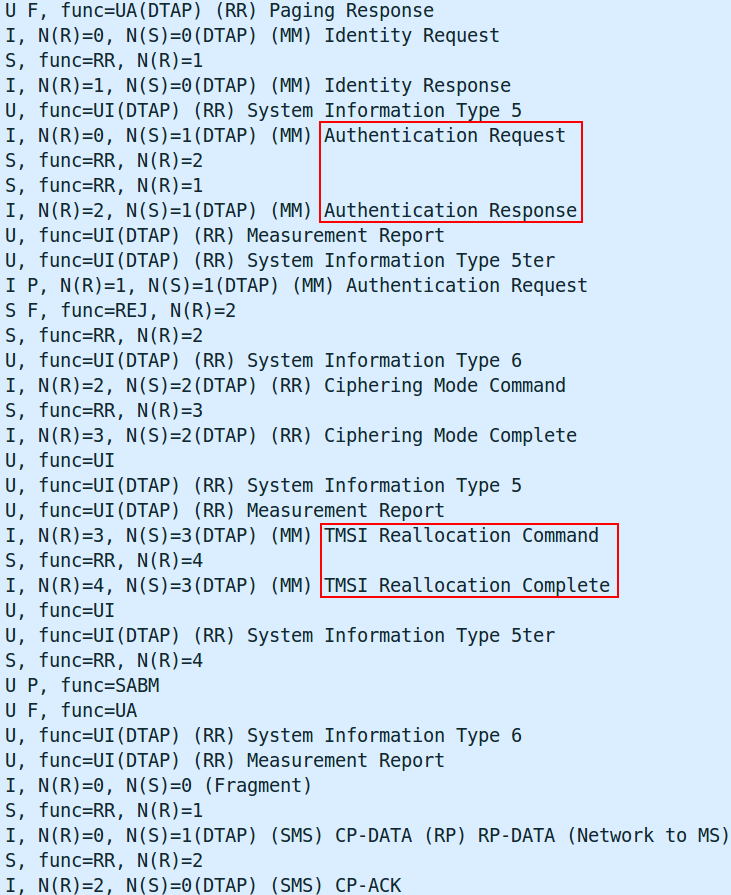
\includegraphics[width=\textwidth]{tmsi_real}
        \caption{TMSI reallocation and rekeying during an MT-SMS on \comp{Telenor}}
        \label{fig:tmsi_real}
      \end{figure}

      Both Norwegian networks are very good on this issue, since they
      trigger a \gls{tmsi} reallocation for each event. It would
      therefore be impossible to use the correlation technique to find
      out the \gls{tmsi} of the target on these networks.

      The data from the \proj{GSM Map} project seems completely outdated
      here, since according to them, \comp{Netcom} only updates the
      \gls{tmsi} $3\%$ of the time and \comp{Telenor} $32\%$. The data
      gathered for this thesis shows that it is closer to $100\%$.

      As a side note, the \gls{tmsi} reallocation in the Location
      Updating Accept messages is always encrypted. So even if an
      attacker could manage to follow all the Immediate Assignment
      messages on a cell, and could manage to record the location
      updating procedure related to the \gls{imsi} of interest, it would
      not be possible to find the related \gls{tmsi} without breaking
      the encryption. The \proj{GSM Map} project offers the same
      conclusion.

    \subsection{Rekeying}

      Since it would be very expensive to crack the A5/1 encryption in
      real time using the Berlin tables set, it is usually necessary to
      find the session key before trying to record a call. Doing so
      relies on the assumption that the session key will not change
      between a first \gls{sms} message used to gather some keystream,
      and the following call. This subject is covered in more details
      in~\Sref{sec:finding_kc}.

      Testing if this assumption holds on Norwegian networks can be done
      by recording the traffic for various network events. This is done
      using \proj{OsmocomBB} and \proj{Wireshark} with the two Belgian
      \gls{sim} cards roaming on the two Norwegian networks. As in the
      previous section, the events recorded are the \glspl{moc}, the
      \glspl{mtc}, the \gls{mo-sms} messages, and the \gls{mt-sms}
      messages. Again, every measure was taken at least three times. An
      example of an \gls{mt-sms} on \comp{Telenor} is given
      on~\fref{fig:tmsi_real}.

      \begin{table}[h]
        \centering
        \begin{tabular}{@{}lllll@{}}
          \toprule
          Operator          & MTC & MOC & MT SMS & MO SMS \\
          \midrule
          Telenor (Base)    & Yes & Yes & Yes    & Yes    \\
          Netcom (Proximus) & No  & No  & No     & No     \\
          \bottomrule
        \end{tabular}
        \caption{Authentication procedure during various events}
        \label{tab:events_authentication}
      \end{table}

      When using the \comp{Base} \gls{sim} roaming on \comp{Telenor},
      every event triggers an authentication procedure and negotiates a
      new key. Thus, the session key is not reused and is limited to one
      session, making it impossible to crack it beforehand. When using
      the \comp{Proximus} \gls{sim} roaming on \comp{Netcom}, most
      events do not initiate an authentication procedure. The one which
      do seem to be the first of their kind after an \gls{imsi} attach.
      According to the \proj{GSM Map} project, both \comp{Telenor} and
      \comp{Netcom} authenticate almost $100\%$ of these events, but
      this does not correspond with the data presented here.

    \subsection{Known plaintext}

      Cracking the A5/1 encryption requires some keystream, and to find
      it, it is necessary to find known plaintext on the encrypted
      traffic. According to the \proj{GSM Map} project, the most
      important plaintext to look at are the frames padding, especially
      for the empty frames, and the System Information messages. The
      usual setup of \proj{OsmocomBB} and \proj{Wireshark} is used again
      to listen to the traffic, and the results are available
      in~\tref{tab:plaintext}.

      \begin{table}[h]
        \centering
        \begin{tabular}{@{}llll@{}}
          \toprule
          Operator & \parbox[t]{2.2cm}{Empty frames\\ padding} & SI6
          padding & \parbox[t]{1.7cm}{Random SI\\ pattern}\\
          \midrule
          Telenor (Base)    & Yes   & Yes & No    \\
          Netcom (Proximus) & Most  & No  & No    \\
          \bottomrule
        \end{tabular}
        \caption{Availability of known plaintext}
        \label{tab:plaintext}
      \end{table}

      The \comp{Telenor} network randomizes the empty frames, except for
      the last byte which is always set to \code{0x2B} in the empty frames
      after the Ciphering Mode Command message. The SI6 messages padding
      is randomized, but it stays the same for two or three messages
      before changing. Anyway, most of the information contained in the
      System Information messages is constant and is thus a great source
      of known plaintext. A solution would be to randomize the pattern
      with which the System Information messages are sent, but this is
      not done in this case. Therefore, it is easy to know which
      encrypted message contains a SI5 for example, and it is also easy
      to know what this message contains.
      
      The \comp{Netcom} network randomizes most of the empty frames
      padding, but some of them are still padded with the \code{0x2B}
      bytes. The SI6 messages are also padded with the \code{0x2B} byte,
      and this is shown on~\fref{fig:netcom_padding}. Most importantly,
      the System Information message pattern is not randomized, and this
      can be seen on~\fref{fig:netcom_dl_sacch} which displays the
      downlink \gls{sacch} on a \comp{Netcom} cell. This makes the SI5
      message a good target. It it thus easy to find known plaintext on
      Norwegian networks, and these observations are consistent with the
      information found in the \proj{GSM Map} project report.

      \begin{figure}
        \centering
        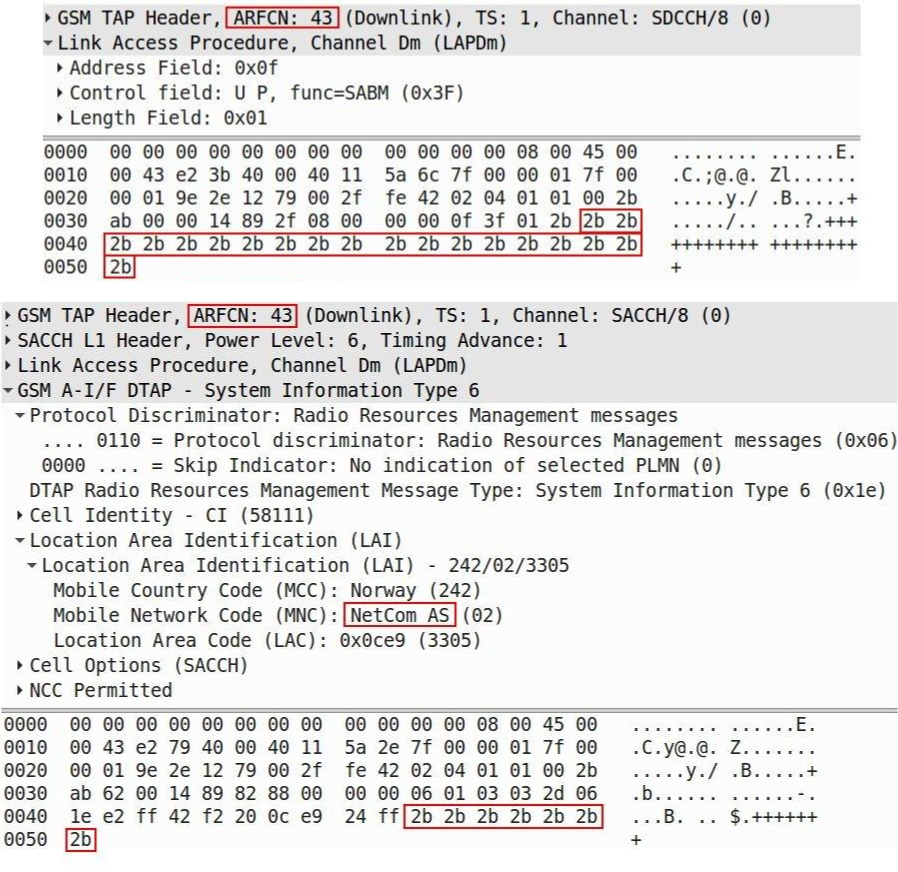
\includegraphics[width=\textwidth]{netcom_padding}
        \caption{Padding of empty frame and SI6 on \comp{Netcom}}
        \label{fig:netcom_padding}
      \end{figure}

      \begin{figure}
        \centering
        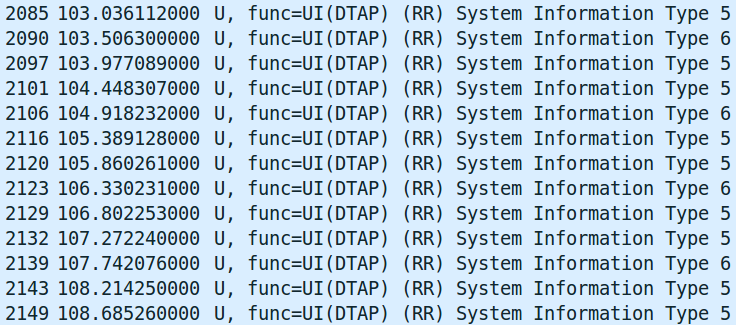
\includegraphics[width=\textwidth]{netcom_dl_sacch}
        \caption{Downlink SACCH on \comp{Netcom}}
        \label{fig:netcom_dl_sacch}
      \end{figure}

      \iffalse
      When using
      the \comp{Proximus} \gls{sim} roaming on \comp{Netcom}. The SI6
      padding are not randomized, but they mostly send the same data
      every time so… The SI5 padding are not randomized either, but the
      contain the list of ARFCN. Anyway, it does not change either. The
      thing that changes a bit more often is the SACCH header containing
      the power level and the timing advance. This might change when the
      targeted \gls{ms} moves, but it mostly stays the same.

      The 2b byte appears in $up func=sabm$, in $si6$, in
      $rp-data(sms)$, in $s, func=rr, n(r)=1$, $sms cp-ack$, in $uf,
      func=ua$, in $rp-ack(sms)$, in $s, func=rr n(r)=3$. 

      The si are not randomized, it is easy to find the pattern. one
      si6 and two si5 on the downlink sacch.

      When using the \comp{Base} \gls{sim} roaming on \comp{Telenor}.
      The position of the SI messages is not random: 5 5ter 6. The si
      messages are mostly constant, so great way to easily find
      keystream. The padding of the si6 changes every two or three
      messages. So this leaves all the si5 and 5ter, and a good part
      of the si6.

      the 2b byte appears in location updating request, auth request
      and id request, also ciph mod comd, cm service request. but not
      encrypted.

      also in location updating accept, channel release, tmsi
      reallocation command, cp ack sms, rp ack sms. 
      also in ,$u func=ui$, $uf func=ua$,  But it is
      always the last one, and the rest is randomized. 

      This does not really matter. As long as you get the si5 for
      example. It is mostly constant and always follows the same
      pattern on the sacch. Also alway sent unencrypted and encrypted,
      so easy to find and xor.
      \fi

    \subsection{Encryption in use}

      Before starting the encryption, the network will first ask the
      phone which algorithm it supports. The phones supported by
      \proj{OsmocomBB} provide A5/1 or A5/2 encryption, but do not
      provide A5/3 encryption. It is therefore not possible to advertise
      its support without modifying the code. The patch is available in
      the appendices \Sref{app:patches} and provides the
      \prog{encryption} command in the \prog{mobile} application of
      \proj{OsmocomBB}, and an example of its use is show in
      \fref{fig:mobile_encryption}. The network decides which encryption
      algorithm to use based on the phone capabilities, and sends its
      decision in the Ciphering Mode Command message.

      \begin{figure}[h]
        \centering
        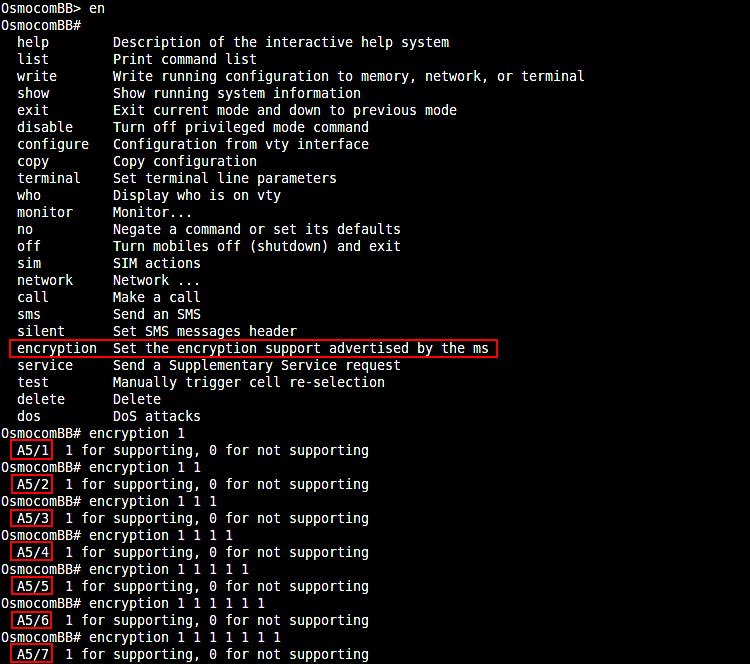
\includegraphics[width=\textwidth]{mobile_encryption}
        \caption{Setting the advertised encryption support using the patched
        \prog{mobile} application}
        \label{fig:mobile_encryption}
      \end{figure}
      

      \begin{table}[h]
        \centering
        \begin{tabular}{@{}lllll@{}}
          \toprule
          Operator          & A5/0  & A5/1 & A5/2 & A5/3 \\
          \midrule
          Telenor (Base)    & No    & Yes & No    & Yes  \\
          Netcom (Proximus) & No    & Yes & No    & Yes  \\
          \bottomrule
        \end{tabular}
        \caption{Use of encryption algorithm}
        \label{tab:plaintext}
      \end{table}

      Both \comp{Telenor} and \comp{Netcom} will refuse an \gls{imsi}
      attach when the \gls{ms} only advertises A5/2 or if the \gls{ms}
      does not support any encryption. An example is show
      on~\fref{fig:telenor_a52}. The cause for the Location Updating
      Reject message is \emph{network failure}. Both networks still
      allow the use of A5/1 when the phone requests it, and both use
      A5/3 when the phone advertises its support. This is shown on
      \fref{fig:netcom_a51} and \fref{fig:netcom_a53}. This is
      consistent with the data provided by the \proj{GSM Map} project.

      \begin{figure}
        \centering
        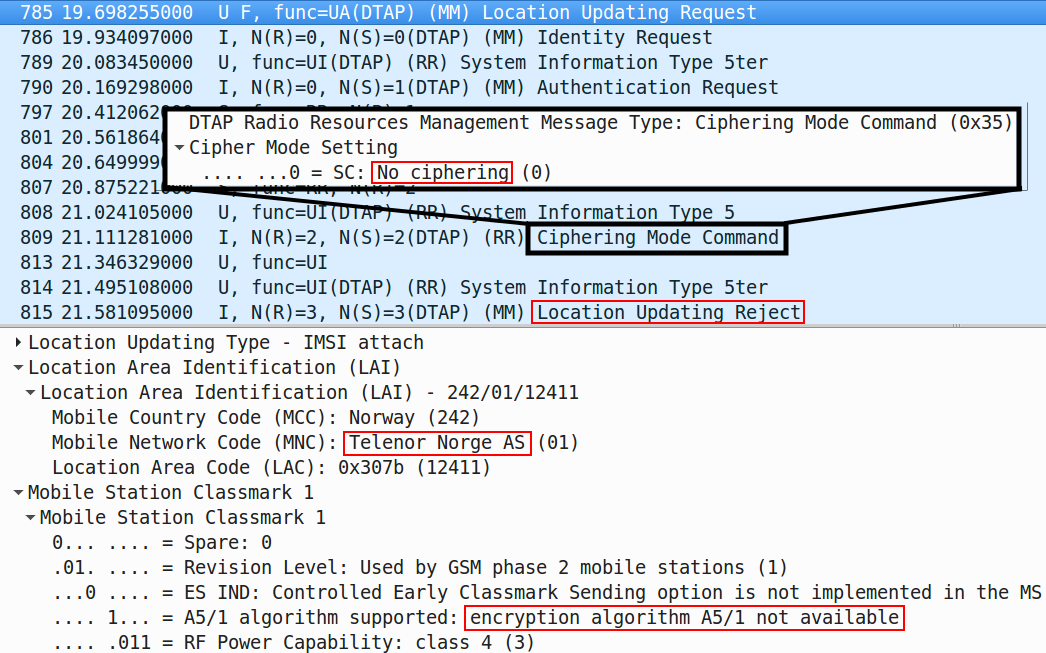
\includegraphics[width=\textwidth]{telenor_a52}
        \caption{Location Updating Reject when \gls{ms} does not
        advertises A5/1 support on \comp{Telenor}}
        \label{fig:telenor_a52}
      \end{figure}

      \begin{figure}
        \centering
        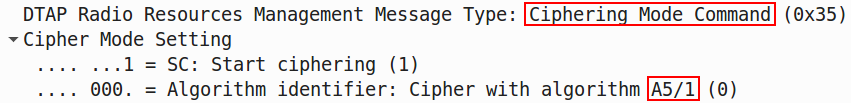
\includegraphics[width=\textwidth]{netcom_a51}
        \caption{Ciphering Mode Command with A5/1 on \comp{Netcom}}
        \label{fig:netcom_a51}
      \end{figure}

      \begin{figure}
        \centering
        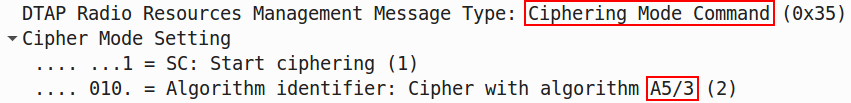
\includegraphics[width=\textwidth]{netcom_a53}
        \caption{Ciphering Mode Command with A5/3 on \comp{Netcom}}
        \label{fig:netcom_a53}
      \end{figure}

      \iffalse
      While \comp{Netcom} asks the \gls{ms} for its capabilities on
      every \gls{imsi} attach, it is not the case for \comp{Telenor}.
      Therefore, it might take a while for a phone suddenly advertising
      A5/3 support instead of A5/1 to benefit from the stronger
      encryption, since the network is not aware of the change.
      \fi

    \subsection{Discussion}

      This concludes the analysis of the \comp{Telenor} and
      \comp{Netcom} networks security in regard to the eavesdropping
      attack introduced in~\Cref{chap:eavesdropping_attacks}. Both
      \comp{Telenor} and \comp{Netcom} seem immune to this attack, even
      though \comp{Netcom} could do a few things better.

      Indeed, the \comp{Telenor} network negotiates a new key for every
      service and it would be very expensive to break the A5/1 key
      instantaneously. This would still be possible though, since known
      plaintext is available. The \comp{Netcom} network, on the other
      hand, does not seem to renegotiate a key for every service, and
      known plaintext is available for this network as well. This makes
      it possible to break the A5/1 encryption and use the key for other
      sessions.

      Still, both networks provide A5/3, and most new phones support it
      as well, which makes this threat irrelevant. Moreover, it would be
      impossible for an attacker to uncover the \gls{tmsi} of the target
      using the correlation method, since it is renegotiated for every
      service on both networks. So, the eavesdropping attack would
      probably not work in Norway considering that most of the
      assumptions on which it was based do not hold.

  \section{Denial-of-Service attacks}

    On the four \gls{dos} attacks introduced in~\Cref{chap:dos_attacks},
    three were implemented for this thesis. On these three attacks, two
    might cause serious damage, and were therefore not tested on a live
    network. The only attack tested in a live environment is the
    \gls{imsi} detach attack, which targets one single individual. Thus,
    this section will only focus on the results of this last attack.

    \subsection{IMSI detach}

      To test this attack, all the available \gls{sim} cards were
      connected to their respective network using various phones. The
      targeted phones do not receive any messages from the network and
      it was therefore not necessary to use \proj{OsmocomBB} to listen
      to the received traffic. The tests were done in four steps.
      Firstly, by contacting every targeted phones to make sure they are
      reachable. Secondly, by sending \gls{imsi} Detach Indication
      messages to all the targeted phones using a phone running the
      modified version of \proj{OsmocomBB}. Thirdly, by trying to
      contact the targeted phones again to make sure they can be
      reached. And finally, by rebooting the targeted phones to trigger
      a location update procedure, and try to contact them again.

      \begin{table}[h]
        \centering
        \begin{tabular}{@{}ll@{}}
          \toprule
          Operator             & IMSI detach\\
          \midrule
          Telenor              & Yes  \\
          Netcom               & No   \\
          Base (On Telenor)    & Yes  \\            
          Proximus (On Netcom) & No   \\
          \bottomrule
        \end{tabular}
        \caption{Effect of the IMSI detach.}
        \label{tab:imsi_detach}
      \end{table}

      The results are shown on~\tref{tab:imsi_detach}. The
      \comp{Telenor} network seems vulnerable to this attack, but the
      \comp{Netcom} network seems to filter these messages. This means
      that, on the \comp{Telenor} network, an attacker could regularly
      send \gls{imsi} Detach Indication messages to a target to prevent
      any contact from the network. An example of \gls{imsi} detach
      message is show on~\fref{fig:telenor_detach} and can be related to
      the command displayed on \fref{fig:mobile_dos_detach}.\fxnote{Need
      to test during a call.}

      \begin{figure}[h]
        \centering
        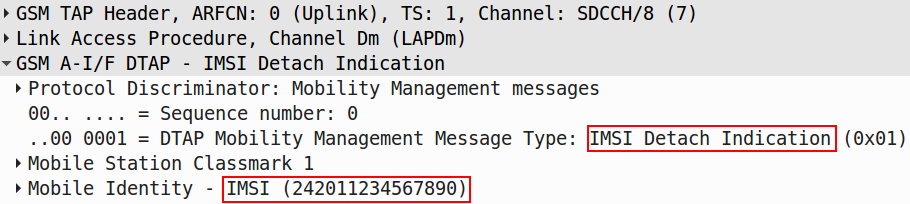
\includegraphics[width=\textwidth]{telenor_detach}
        \caption{IMSI Detach Indication message with an IMSI of
        242011234567890 on \comp{Telenor}}
        \label{fig:telenor_detach}
      \end{figure}


    \iffalse
    NEED TO TEST IMSI DETACH FROM TELENOR TO NETCOM ETC. SEE IF CAN
    DETACH PHONE IN OTHER COUNTRIES AND SO ON.

    The Location Updating Reject can reply either with
    Forbidden PLMN, or IMSI unknown in HLR. I do not know which value of
    the \gls{imsi} triggers the second one, but that's what we want.
    imsi detach as well
    \fi

      \iffalse
     It works well on telenor network but not on netcom's. This
    was tested with the telenor sim, the netcom sim, the proximus sim
    and the base sim. I guess that netcom filter these requests. This
    has a limited effect, as soon as the targeted phone contacts the
    network for any reason, it is removed. So when starting the phone
    again, the text message shows up.

    When starting the phone again, the text shows up.
    \fi

    \subsection{Discussion}

      It is difficult to say if the \gls{dos} attacks would be effective
      against Norwegian networks without testing them. The RACHell
      attack seems very difficult to prevent, but is limited to one
      cell. The \gls{imsi} attach flood attack seems hard to prevent as
      well, considering that the \gls{imsi} of the phone can be changed
      for every request. One solution would be to isolate the cell where
      the \gls{dos} originates from the rest of the network. This would
      prevent legitimate users in that cell to access the network but
      would limit the damages. It would be interesting to know if
      \comp{Telenor} or \comp{Netcom} have any solutions in
      place.\fxnote{Contact them?}

      The \gls{imsi} detach attack is not effective on the \comp{Netcom}
      network, which probably filters the IMSI Detach Indication
      messages altogether since they are not essential to the network
      operation. The \comp{Telenor} network is vulnerable, as long as
      the attacker knows the \gls{imsi} or the \gls{tmsi} of the target.
      But on both Norwegian networks, the \gls{hlr} queries do not
      return a valid \gls{imsi}, and the \gls{tmsi} is reallocated for
      every transaction. This makes the \gls{imsi} detach attack much
      more complicated in practice.
